\documentclass[specification,annotation,times]{itmo-student-thesis}

%% Опции пакета:
%% - specification - если есть, генерируется задание, иначе не генерируется
%% - annotation - если есть, генерируется аннотация, иначе не генерируется
%% - times - делает все шрифтом Times New Roman, требует пакета pscyr.

%% Делает запятую в формулах более интеллектуальной, например:
%% $1,5x$ будет читаться как полтора икса, а не один запятая пять иксов.
%% Однако если написать $1, 5x$, то все будет как прежде.
\usepackage{icomma}

%% Данные пакеты необязательны к использованию в бакалаврских/магистерских
%% Они нужны для иллюстративных целей
%% Начало
\usepackage{tikz}
\usetikzlibrary{arrows}
\usepackage{placeins}
% \usepackage{filecontents}

%% Конец

%% Указываем файл с библиографией…
\addbibresource{thesis.bib}

%% …и папку с рисунками.
\graphicspath{ {../Images/} }

\begin{document}

%% Метаданные об авторе и работе. Нужны для генерации титульника,
%% аннотации и задания.
\studygroup{M4239}
\title{Разработка алгоритмов статического поиска выходов за пределы
    динамического массива в С/C++ программах}
\author{Громаковский Иван Евгеньевич}{Громаковский И.Е.}
\supervisor{Лукин Михаил Андреевич}{Лукин М.А.}
    {канд. техн. наук}{тьютор кафедры КТ Университета ИТМО}
\publishyear{2017}
%% Дата выдачи задания. Можно не указывать, тогда надо будет заполнить от руки.
\startdate{01}{сентября}{2015}
%% Срок сдачи студентом работы. Можно не указывать, тогда надо будет заполнить от руки.
\finishdate{31}{мая}{2017}
%% Дата защиты. Можно не указывать, тогда надо будет заполнить от руки.
%% \defencedate{15}{июня}{2015}

%% \addconsultant{Белашенков Н.Р.}{канд. физ.-мат. наук, без звания}
%% \addconsultant{Беззубик В.В.}{без степени, без звания}

%% Задание
%%% Техническое задание и исходные данные к работе
\technicalspec{Требуется разработать и реализовать алгоритм
  статического поиска выходов за пределы динамического массива в C/C++
  программах. Необходимо обрабатывать промышленные программы больших
  размеров (состоящие из сотен тысяч строк) за разумное время (порядка
  нескольких десятков минут). Анализатор должен находить как можно
  больше ошибок с как можно меньшим числом ложных срабатываний. На
  сегодняшний день известно множество свободно распространяемых
  анализаторов, решающих аналогичную или более общую проблему. В
  данной работе необходимо также произвести сравнение с другими
  анализаторами.}

%%% Содержание выпускной квалификационной работы (перечень подлежащих разработке вопросов)
\plannedcontents{\begin{enumerate}
    \item Обоснование актуальности задачи, описание предметной
      области, обзор существующих решений.
    \item Теоретическое исследование задачи поиска выходов за пределы
      динамического массива в C/C++. Разработка алгоритма.
    \item Описание практической реализации алгоритма, результаты
      экспериментов, сравнение с другими анализаторами.
\end{enumerate}}

%%% Исходные материалы и пособия
\plannedsources{\begin{enumerate}
    \item Li, Lian, Cristina Cifuentes, and Nathan Keynes. "Practical
      and effective symbolic analysis for buffer overflow detection."
      Proceedings of the eighteenth ACM SIGSOFT international
      symposium on Foundations of software engineering. ACM, 2010.
    \item Shahriar, Hossain, and Mohammad Zulkernine. "Classification
      of static analysis-based buffer overflow detectors." Secure
      Software Integration and Reliability Improvement Companion
      (SSIRI-C), 2010 Fourth International Conference on. IEEE, 2010.
    \item Le, Wei, and Mary Lou Soffa. "Marple: a demand-driven
      path-sensitive buffer overflow detector." Proceedings of the
      16th ACM SIGSOFT International Symposium on Foundations of
      software engineering. ACM, 2008.
    \item Ding, Sun, et al. "Detection of buffer overflow
      vulnerabilities in C/C++ with pattern based limited symbolic
      evaluation." Computer Software and Applications Conference
      Workshops (COMPSACW), 2012 IEEE 36th Annual. IEEE, 2012.
\end{enumerate}}

%%% Календарный план
\addstage{Ознакомление с основами статического анализа}{10.2015}
\addstage{Изучение существующих подходов к решению данной проблемы}{02.2016}
\addstage{Разработка и реализация прототипа анализатора}{06.2016}
\addstage{Исследование преимуществ и недостатков прототипа,
  разработка теоретических улучшений}{11.2016}
\addstage{Реализация улучшенной версии анализатора}{01.2017}
\addstage{Проведение экспериментов, сравнение с другими анализаторами}{02.2017}
\addstage{Написание пояснительной записки}{05.2017}

%% Аннотация
%%% Цель исследования
\researchaim{Разработка алгоритмов статического анализа C/C++ программ
  для поиска выходов за пределы динамического массива.}

%%% Задачи, решаемые в ВКР
\researchtargets{\begin{enumerate}
    \item способность находить как можно больше ошибок, связанных с
      выходами за пределы динамического массива, с как можно меньшим
      числом ложных срабатываний;
    \item обработка крупных промышленных приложений, состоящих из
      сотен тысяч строк, за разумное время;
    \item проведение экспериментов, сравнение с другими анализаторами.
\end{enumerate}}

%%% Использование современных пакетов компьютерных программ и технологий
\advancedtechnologyusage{Анализатор был реализован на языке C++ с
  использованием системы сборки CMake. Использовалась инфраструктура
  LLVM. Также использовались библиотеки Boost и STL. Для анализа
  больших программ использовалась утилита whole-program-llvm. Также
  были написаны Bash-скрипты для упрощения запуска приложения и
  автоматизации. Использовалась система контроля версий Git. Для
  написания пояснительной записки использовался \LaTeX.}

%%% Краткая характеристика полученных результатов
\researchsummary{В результате получился анализатор, способный находить
  ошибки в больших программах за разумное время и превосходящий
  существующие анализаторы, такие как PVS-Studio, в некоторых случаях
  (т. к. сравнение в общем случае невозможно).}

%%% Гранты, полученные при выполнении работы
\researchfunding{Грантов или других форм государственной поддержи и
  субсидирования в процессе работы не предусматривалось.}

%%% Наличие публикаций и выступлений на конференциях по теме выпускной работы
\researchpublications{
  \begin{refsection}
  \nocite{kmu-russian,kmu-english}
  \printannobibliography
  \end{refsection}
}


%% Эта команда генерирует титульный лист, задание и аннотацию.
\maketitle{Магистр}

%% Оглавление
\tableofcontents

%% Макрос для введения. Совместим со старым стилевиком.
\startprefacepage

%% В этом файле написано введение.
% -*-coding: utf-8-*-

Программное обеспечение всегда было и остаётся подвержено
ошибкам. Одними из наиболее уязвимых являются программы, написанные на
языках C и C++, поскольку они предоставляют прямой доступ к памяти и
не имеют встроенных механизмов для предотвращения некорректного
обращения к памяти. Пожалуй, наибольшую опасность представляют ошибки,
при которых происходит доступ к памяти (чтение или запись) за
пределами выделенного буфера. Такие ошибки могут приводить как к
остановке программы, так и к более серьёзным проблемам с точки зрения
безопасности. Например, злонамеренный пользователь может получить
доступ к приватной информации, исполнить произвольный код, а в худшем
случае получить права суперпользователя~\cite{onesmashing}.

Существует большое число подходов к решению данной проблемы, как
статических~\cite{wagner2000first, xie2003archer, ganapathy2003buffer,
le2008marple, li2010practical}, так и
динамических~\cite{cowan1998stackguard,
ruwase2004practical}. Динамические подходы обнаруживают ошибки во
время работы программы и имеют несколько серьёзных недостатков по
сравнению со статическими подходами, когда программа анализируется до
запуска. Во-первых, дополнительные проверки, выполняемые во время
работы программы, занимают какое-то время и тем самым ухудшают
производительность. Во-вторых, даже если ошибка будет обнаружена,
программа в лучшем случае просто остановится. В-третьих, зачастую
оказывается довольно сложно быстро внести изменения, направленные на
исправление ошибок, и донести их до конечного пользователя. Поэтому
гораздо предпочтительнее обнаружить ошибки до поставки программы
пользователю.

Основная цель данной работы состоит в разработке алгоритмов
статического анализа C/C++ программ на предмет выхода за пределы
динамического массива. При этом необходимо обрабатывать большие
программы, состоящие из сотен тысяч строк, за разумное время. В общем
случае задача поиска всех выходов за пределы массива без единого
ложного срабатывания неразрешима, поэтому анализатор должен находить
как можно больше реальных ошибок, при этом выдавая как можно меньше
ложных срабатываний.

За основу данной работы был взят подход, описанный в
статье~\cite{li2010practical}. Были выявлены преимущества и недостатки
подхода, предложены и реализованы способы решения найденных
недостатков. С помощью проделанных улучшений удалось существенно
уменьшить число ложных срабатываний, тем самым увеличив точность
анализа. Также было проведено сравнение с другими свободно
распространяемыми анализаторами, показано превосходство над
ними. Реализованный алгоритм способен обрабатывать программы,
состоящие из сотен тысяч строк, за время порядка десяти минут.

В первой главе приведён обзор предметной области и существующих
решений описанной проблемы. Во второй главе представлены результаты
исследования алгоритма из статьи~\cite{li2010practical}, описан
теоретический подход к устранению выявленных недостатков. В третьей
главе рассмотрены вопросы практической реализации предложенного
решения, приведены основные результаты работы и сравнение с другими
анализаторами.


%% Начало содержательной части.
%% В этих файликах находятся главы из содержательной части.

%-*-coding: utf-8-*-
\chapter{Обзор предметной области}

\section{Описание проблемы}

Ошибки в коде программного обеспечения могут представлять большую
опасность и приводить с серьёзным убыткам. Например, в 2003-ем году
большое число компьютеров по всему миру было заражено вирусом SQL
Slammer~\cite{moore2003spread}, что приводило к отказу оборудования и
существенному замедлению трафика в сети Интернет в целом. Другим
примером служит червь Code-Red, убытки от которого оцениваются
миллиардами долларов~\cite{moore2002code}. Оба вируса использовали
уязвимости в программном коде, позволявшие осуществить выход за
пределы массива. Такие ошибки являются одними из наиболее опасных,
поскольку зачастую злоумышленик может, используя уязвимость, выполнить
произвольный код и/или получить права
суперпользователя~\cite{onesmashing}.

Наиболее актуальна данная проблема для языков C/C++. Дизайн этих
языков подразумевает высокую гибкость и производительность, жертвуя
безопасностью. Языки позволяют осуществлять произвольный доступ к
памяти и не имеют встроенных автоматических проверок корректности. Для
многих приложений данный недостаток является менее существенным, чем
производительность, поэтому языки C и C++ активно используются и по
сей день. Также порой выбор языка происходит по историческим
соображениям, когда приходится поддерживать старый код. Многие
операционные системы написаны на C/C++ из соображений гибкости и
производительности. Также существует большое число программ,
работающих с сетью и получающих данные извне, написанных на C/C++ из
соображений производительности. Уязвимости в таком программном
обеспечении являются крайне опасными, поскольку операционные системы
работают напрямую с аппаратными средствами, а ошибки в сетевых
приложениях могут быть эксплуатированы удалённо фактически любым
человеком.

В данной работе под выходом за пределы динамического массива
подразумевается обращение (чтение и запись) к памяти за пределами
выделенного участка памяти. Если существуют такие входные данные (то
есть любые данные, неизвестные заранее), что при запуске программы с
этими данными в ней присутствует инструкция, совершающая
выход за пределы массива, то такая инструкция считается ошибочной и
потенциально уязвимой. Задача состоит в поиске таких инструкций.

В связи с актуальностью проблемы ей уделено большое внимание учёных и
инженеров по всему миру. Известно большое число подходов к решению
данной задачи. Глобально их можно разделить на динамические и
статические.

Динамические подходы~\cite{cowan1998stackguard, ruwase2004practical,
  hastings1991purify} состоят в добавлении в программу дополнительных
проверок, предотвращающих обращение к памяти за пределами выделенного
буфера. Основное преимущество этого подхода в том, что он, как
правило, предотвращает большее число ошибок, поскольку значения всех
переменных известны в момент обращения к памяти. Однако такие подходы
существенно замедляют работу программы, что зачастую оказывается
неприемлимо в случаях, когда производительность стоит на первом
месте. Другим недостатком динамического подхода является тот факт, что
при наличии ошибки она будет обнаружена уже во время программы, что,
скорее всего, приведёт к остановке. Также динамические подходы
способны находить лишь ошибки, которые воспроизводятся на реально
выполняемых участках кода. На практике же нередко происходит так, что
какой-то фрагмент кода может не выполняться на протяжении очень
длительного времени, однако именно в нём может быть ошибка, которая
очень долго будет оставаться незамеченной.

Статический анализ, в отличие от динамического, производится без
запуска программы. Это позволяет исследовать все места в коде, даже
редко выполняемые, а также позволяет найти ошибки до реального
использования программы, пока они не проявили себя. Помимо этого
статический анализ никак не меняет исполняемый код, а значит, не
замедляет программу. В общем случае задача поиска всех выходов за
пределы массива в C/C++ без единого ложного срабатывания неразрешима
(это напрямую следует из проблемы
останова~\cite{turing1937computable}), поэтому одним из главных
недостатков статического анализа является необходимость ручного
рассмотрения результатов работы анализатора с целью выяснения, какие
из найденных ошибок действительно являются таковыми.

Таким образом, динамические и статические подходы имеют свои
преимущества и недостатки. В разных случаях имеет смысл применять
разные подходы (в том числе комбинацию подходов). Оба варианта
являются осмысленными и актуальными. В данной работе был сделан выбор
в пользу статического анализа. Поскольку задача неразрешима в общем
случае, требуется находить как можно больше ошибок в программах,
минимизируя при этом число ложных срабатываний. Важным требованием
является способность обрабатывать крупные программы, состоящие из
сотен тысяч строк, за разумное время. Как правило, приемлимым является
время порядка нескольких десятков минут. Это сопоставимо со временем
сборки проекта и позволяет, например, включить анализатор в систему
непрерывной интеграции.

Несмотря на огромное число исследований, посвящённых данной проблеме,
уязвимости, связанные с выходом за пределы массива продолжают
оставаться одними из наиболее часто встречаемых~\cite{uscert}. Таким
образом, на сегодняшний день задача не перестаёт быть
актуальной. Также стоит отметить, что большое число подходов,
описанных в статьях, находятся в закрытом доступе или же
поддерживаются на протяжении долгих лет. Большинство доступных
анализаторов решают более общую проблему поиска различных ошибок и
либо работают слишком долго на больших программах, либо находят
слишком мало ошибок, связанных с выходами за пределы массива.

\section{Обзор существующих решений}

Существует больше число статей, посвящённых статическому поиску
выходов за пределы динамического массива в C и C++. Отдельно стоит
отметить статью~\cite{shahriar2010classification}, в которой
представлена классификация различных подходов. В большинстве случаев
основной компромисс делается между скоростью работы, числом находимых
ошибок и точностью.

Наиболее простые анализаторы~\cite{viega2002token,flawfinder} не
учитывают поток управления и зависимости по данным в программе, а
выполняют лишь символьный анализ. Такие подходы просты в реализации и
работают очень быстро, однако точность анализа крайне низкая. По сути,
такие анализаторы лишь находят потенциально опасные места в программе
и эвристически сортируют их. В данной работе требуется большая
точность, поэтому необходимо учитывать семантику программы.

Некоторые подходы~\cite{larochelle2001statically, hackett2006modular,
  dor2003cssv} основаны на использовании пользовательских аннотаций
для вывода ограничений на значения переменных. В таком случае
разработчик пишет аннотации в различных местах в коде. Аннотации
сообщают анализатору различные инварианты, гарантированно
выполняющиеся в определённом месте. Например, что значение переменной
ограничено сверху определённым значением. Анализатор работает в
предположении, что все инварианты, задаваемые аннотациями, выполнены,
что ползволяет повысить точность анализа. Некоторые анализаторы также
проверяют корректность аннотаций. Недостатком таких подходов
является необходимость добавления аннотаций в код. В некоторых случаях
это не представляет большой проблемы, особенно если приложение пишется
с нуля. Однако для больших программ добавление аннотаций к каждой
функции может занять чрезвычайно много времени. Наибольшую трудность
представляет аннотирование старого кода, написанного незнакомыми
людьми. Поскольку основной целью работы является анализ крупных
программ, использование аннотаций не имеет большого смысла, и в этой
работе они не используются.

Также для решения рассматриваемой задачи можно использовать подходы,
базирующиеся на ограниченной проверке моделей (bounded model
checking)~\cite{cordeiro2012smt, merz2012llbmc}. Такой подход
позволяет проверять различные свойства программы, включая наличие
выходов за пределы массива. Для этого программа описывается системой
переходов, проверяемое свойство формулируется в виде логического
утверждения, после чего выполнимость условия проверяется SAT- или
SMT-решателем. При этом рассматриваются пути в программе с
ограниченной глубиной, чтобы гарантировать, что анализ
закончится. Такие подходы обладают хорошей точностью и позволяют
проверять различные свойства программы, однако это достигается за счёт
низкой производительности. Проблема заключается в экспоненциальном
росте сложности задачи при увеличении числа ветвлений в программе. В
результате такие подходы не могут быть применены к большим программам.

Подходы, описанные в статьях~\cite{wagner2000first,
  ganapathy2003buffer, larochelle2001statically}, в целом весьма
похожи. Сначала анализатор обходит весь код программы и строит систему
ограничений на значения переменных. Затем система решается с
использованием различных алгоритмов (зависит от анализатора). В
результате выводится как можно более точная оценка возможных значений
переменных. После этого обращения к массиву анализируются, исходя из
выведенных ограничений. Подходы различаются в основном
чувствительностью анализа (учётом контекста, наличием межпроцедурного
анализа и т. д.), гранулярностью анализа и способом разрешения
ограничений. За счёт различных эвристик такие подходы работают
относительно быстро на программах среднего размера, однако на больших
программах получается слишком много ограничений, и их решение занимает
слишком много времени.

В статье~\cite{xie2003archer} описан подход, способный обрабатывать
программы, состоящие из сотен тысяч строк кода. Этот подход использует
полностью символьный анализ, в рамках которого возможные значения
переменных представлены символьно, что позволяет учитывать зависимости
между переменными, не зная конкретных значений. Анализ является
межпроцедурным, что существенно повышает точность на практике. При
анализе конкретной функции происходит проход по графу потока
управления всей функции. Каждая инструкция может модифицировать
контекст анализатора. При обработке условных переходов выполняется
проверка значения, влияющего на переход. Если значение не может быть
посчитано статически, происходит размножение контекста, и анализатор
продолжает работу с большим числом контекстов. При обработке обращения
к массиву анализатор может непосредственно вывести, возможно ли
переполнение. За счёт отсутствия необходимости разрешать системы
ограничений такой подход работает быстрее предыдущих.

Более современная идея заключается в использовании анализа «по
требованию», при котором анализируются только те инструкции программы,
которые влияют на результат какого-то запроса. Например,
статья~\cite{le2008marple} использует анализ по требованию для поиска
выходов за пределы массива. Основная цель данной идеи заключается в
уменьшении числа анализируемых путей программы и, следовательно,
повышении скорости анализа. «Требование» анализа возникает в местах,
где может выполниться какой-то запрос (в данном случае в местах
обращения к массиву). Затем происходит распространение запроса в
обратном направлении по графу потока управления. В процессе
распространения происходит сбор информации о значениях переменных,
влияющих на запрос. Обход заканчивается, когда ответ на запрос может
быть однозначно вычислен или при достижении входа в функцию. На
практике такой подход работает существенно быстрее аналогичных
подходов, анализирующих программу целиком. Схожие идеи применены также
в статьях~\cite{ding2012detection, ding2014abor, li2010practical}.

\section{Обзор статьи~\cite{li2010practical}}

На основании проведённого изучения литературы было принято решение
использовать алгоритм, описанный в статье \cite{li2010practical}, в
качестве базового. Во-первых, этот подход является легковесным, что
позволяет достаточно быстро обрабатывать большие программы. Во-вторых,
результаты, представленные в статье, говорят о том, что анализатор
способен находить много ошибок в крупных открытых проектах. В-третьих,
несмотря на довольно хорошие результаты, авторы также отмечают наличие
ложных срабатываний и спорных ситуаций, в которых алгоритм не может
принять однозначное решение. А значит, у этого подхода есть
пространство для улучшений.

\subsection{Static Single Assignment}

Описанный в статье алгоритм рассматривает программу, представленную в
Static Single Assignment форме~\cite{cytron1991efficiently} (SSA). Такое
представление является весьма удобным для статического анализа. SSA
форма имеет две особенности. Во-первых, значение любой переменной
присваивается ровно один раз. Во-вторых, вводится специальная
инструкция $\phi$, возвращающая один из своих аргументов в зависимости
от того, из какого предка поток управления пришёл в эту инструкцию. За
счёт этого удаётся представить различные языковые конструкции, при
которых происходит изменение значения переменной, например, циклы.

\begin{figure}
    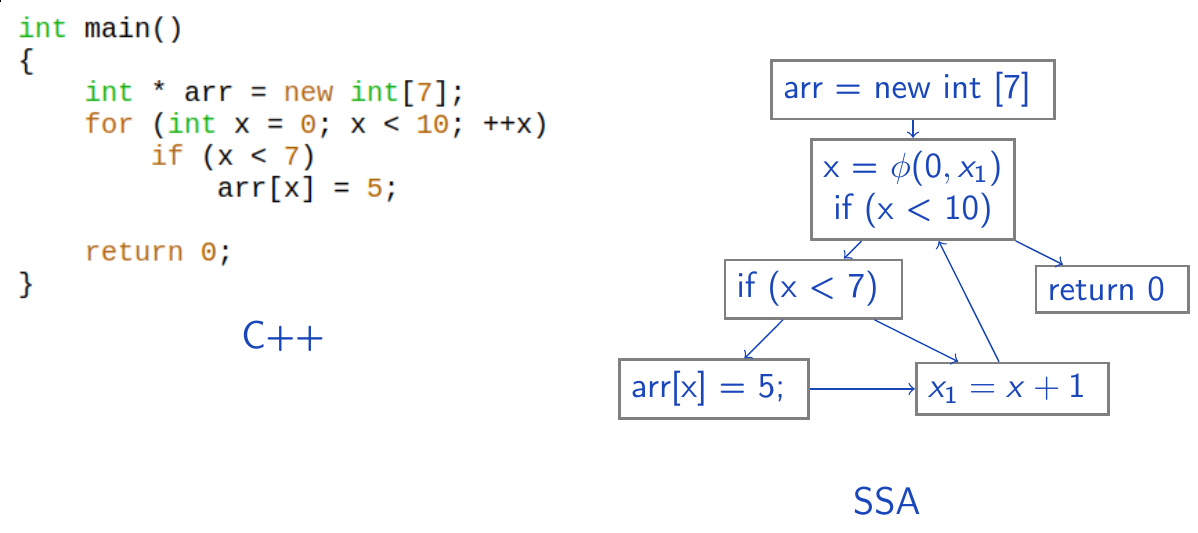
\includegraphics[width=\textwidth]{ssa.png}
    \caption{SSA форма}
    \label{fig:ssa}
\end{figure}

На рисунке~\ref{fig:ssa} представлен пример SSA формы. В C++ программе
значение переменной $x$ меняется на каждой итерации цикла. Однако в
SSA форме значение переменной может присваиваться только один раз. Для
этого значение $x$ определяется как $\phi$ от начального значения
($0$) и дополнительной переменной $x_1$, определённой как $x +
1$. Таким образом, на каждой итерации цикла значение переменной $x$
будет на 1 больше предыдущего, что соответствует C++ коду.

\subsection{Символьные вычисления}

Алгоритм базируется на символьных вычислениях для обнаружения выходов
за пределы массива. Символьные вычисления позволяют учесть зависимости
между переменными, не зная их численных значений. В основе алгоритма
лежит понятие символьного выражения (symbolic expression), а также
символьного диапазона (symbolic range).

Символьным выражением может быть число, переменная, афинная функция
другого символьного выражения, а также два специальных значения $\bot$
и $\top$, соответствующих наименьшему и наибольшему возможному
значению. Для символьных выражений естественным образом определяются
операции сложения, вычитания, умножения и деления. Также вводится
частичный порядок ($\prec$) следующим образом: $E_1 \prec E_2$ тогда и
только тогда, когда $E_1 - E_2$ не больше нуля (для всех непостоянных
значений).

Символьный диапазон определяется как пара символьных выражений. Для
символьных диапазонов также определяются операции сложения, вычитания,
умножения и деления. К ним добавляются операции пересечения и
объединения. Для переменной $V$ вводится понятие define range $S_V$
--- символьного отрезка, соответствующего диапазону возможных значений
$V$ в месте её определения. Так как программа представлена в SSA
форме, определение переменной и присвоение ей значения происходит
ровно в одном месте. Также вводится понятие use range для переменной
$V$ и инструкции $P$: $S_{V,P}$. Этот символьный диапазон
соответствует возможным значениям $V$ в месте инструкции $P$. Такой
диапазон может отличаться от define range, поскольку на пути к
инструкции $P$ могут быть условные переходы с предикатами,
ограничивающими значение $P$.

\subsection{Вычисление диапазонов}

Для расчёта описанных выше диапазонов рассматриваются два вида
зависимостей: зависимости по данным и зависимости потока управления.

Зависимости по данным используются для расчёта define range $S_V$, то
есть диапазона возможных значений $V$ в месте определения. Он
вычисляется через use range аргументов в инструкции, определяющей
$V$. Например, если $V = a + b$, то $S_V = S_{a, V} + S_{b, V}$. Для
$V = \phi(a, b)$ используется объединение, поскольку $\phi$ может
вернуть любой из аргументов: $S_V = S_{a, V} \cup S_{b, V}$. Аналогично
вычисляется define range для других инструкций.

Зависимости потока управления используются для уточнения диапазона
значений переменной $V$ в инструкции $P$ ($S_{V, P}$), который может
отличаться от $S_V$. Для уточнения используются условные переходы,
лежащие на путях $P$, в которых используются предикаты, затрагивающие
$V$. При этом рассматриваются только условные переходы,
удовлетворяющие двум условиям. Во-первых, узел, соответствующий $P$ в
графе потока управления, должен доминироваться узлом, соответствующим
условному переходу. Другими словами, любой путь из входа в функцию в
инструкцию $P$ должен проходить через рассматриваемый условный
переход. Во-вторых, $P$ должна быть достижима только из одного потока
условного перехода. В таком случае условие, соответствующее этому
потомку, считается выполненым, и применяется для уточнения диапазона
значений $V$. Например, для условия $V \geq y$ диапазон значений $V$
будет пересечён с $[y, \top]$. Также учитываются предикаты, в которых
$V$ фигурирует не напрямую, а через афинное преобразование. Например,
$2 * V + 3 < W$. В этом случае диапазон будет пересечён с $[\bot,
\frac{W - 3}{2}]$.

Выход за пределы массива размера $n$ при обращении по индексу $index$
(инструкция $P$) фиксируется, если
$S_{n, P}^{max} \prec S_{index, P}^{max}$, то есть максимальная оценка
размера меньше либо равна максимальной оценки индекса, или $S_{index, P}^{min} \prec
-1$, то есть индекс может быть отрицательным. Если $S_{index, P}^{max}
\prec S_{n, P}^{min} - 1$ и $0 \prec S_{V, P}^{min}$, то выход за
пределы массива точно не может случиться. В остальных случаях алгоритм
не может однозначно определить, возможно ли переполнение. В таких
случаях алгоритм не сообщает об ошибке, поскольку это приводило бы к
слишком большому числу ложных срабатываний, и анализатором было бы
очень сложно пользоваться.

Алгоритм использует идею анализа «по требованию». Вычисление
диапазонов значений начинается в инструкциях, в которых происходит
непосредственное обращение к массиву. Для проверки корректности
вычисляются диапазоны значений размера массива и индекса, по которому
производится обращение. Поскольку в графе зависимостей между
переменными могут присутствовать циклы, используется специальный
итерационный алгоритм, гарантирующий прогресс и итоговое завершение
работы анализатора (итерации выполняются до достижения неподвижной
точки).

\chapterconclusion

В данной главе была подробно описана проблема выхода за пределы
динамического массива в C/C++ программах, показана её
актуальность. Был приведён обзор существующих решений этой проблемы,
описаны ключевые характеристики различных статических
подходов. Наиболее оптимальными, с точки зрения производительности,
являются подходы, использующие анализ «по требованию». Также был обоснован
выбор алгоритма из статьи~\cite{li2010practical} в качестве базового
подхода для данной работы, приведён более подробный обзор этого
алгоритма.

\FloatBarrier

%-*-coding: utf-8-*-
\chapter{Теоретическое исследование}

В данной работе было проведено подробное исследование подхода,
представленного в статье~\cite{li2010practical}. В связи с отсутствием
реализации описанного алгоритма в открытом доступе он был реализован с
нуля в полном соответствии с приведённом в статье описанием. В ходе
исследования основное внимание было уделено недостаткам этого
подхода. Были выявлены случаи, в которых описанный алгоритм работает
некорректно. Ниже представлено описание таких случаев, а также
предложены способы решения этих проблем.

\section{Обработка циклов}

В данном разделе описаны две проблемы, связанные с обработкой
циклов.

\subsection{Монотонно изменяющиеся переменные}

\begin{figure}
    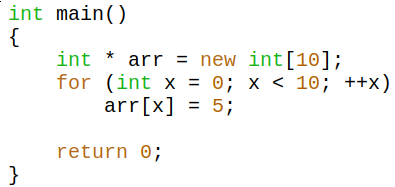
\includegraphics[]{for-trivial.png}
    \caption{Простой цикл: C++}
    \label{fig:for-trivial-cpp}
\end{figure}

\begin{figure}
    \inputTikZ{for-trivial}
    \caption{Простой цикл: SSA форма}
    \label{fig:for-trivial-ssa}
\end{figure}

На рисунке~\ref{fig:for-trivial-cpp} представлен фрагмент C++ кода с
простым циклом, в котором значение переменной $x$ меняется от нуля до
девяти включительно. На рисунке~\ref{fig:for-trivial-ssa} представлена
соответствующая ему SSA форма.

В данном случае алгоритм, описанный в статье~\cite{li2010practical},
будет работать следующим образом. Для проверки корректности записи в
массив будет посчитан диапазон возможных значений переменной $x$ в
месте записи в массив. Для этого сначала будет посчитан диапазон
значений $x$ в месте определения. Изначально в качестве диапазона
будет взят $[\bot, \top]$. Поскольку $x$ выражается как
$\phi$-инструкция, необходимо посчитать диапазон значений $x_1$ в
месте определения $x$ и объединить с $[0, 0]$ (диапазоном значений
второго аргумента). Диапазон значений $x_1$ вычисляется через диапазон
значений $x$ в месте определения $x_1$. Изначально для $x$ был взят
отрезок $[\bot, \top]$, однако в месте определения $x_1$ также будет
применён предикат $x < 10$. Таким образом, диапазон значений $x_1$
будет $[\bot, 10]$. Объединяя его с $[0, 0]$, получаем $[\bot, 10]$ и
для $x$. Это значит, что в данном примере анализатор посчитает, что
$x$ может быть отрицательным, а значит, запись в массив
некорректна. Однако нетрудно видеть, что в действительности это не
так, $x$ не может быть меньше нуля, а запись в массив всегда
корректна. Таким образом, алгоритм выдаёт ложное срабатывание на
данном примере.

Для решения проблемы предлагается использовать дополнительной правило
для вычисления define range. Предположим, что значение $x$ определено
как $\phi(a, b)$, при этом $b = f(x)$. Пусть $f$ удовлетворяет
условию, что последовательность $a, f(a), f(f(a)), \dots$ ---
монотонна (не умаляя общности, предположим, что последовательность
возрастает). Нетрудно видеть, что в таком случае множество возможных
значений $x$ содержится в $\{f^i(a) : i \in [0 .. \inf)\}$ и что все
элементы этого множество не меньше $a$.  Тогда для вычисления define
range $x$ применяется условие $x \geq a$. Примером такой функции $f$
является прибавление или вычитание значения с постоянным знаком.

За счёт использования описанного выше правила в приведённом примере
define range переменной $x$ будет $[0, 10]$, т. к. прибавление единицы
удовлетворяет сформулированному выше условию. Таким образом, в данном
случае удаётся избежать ложного срабатывания.

\subsection{Обработка предиката «не равно»}

\begin{figure}
    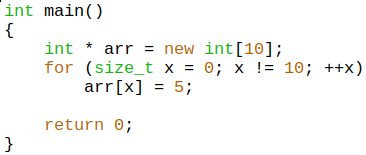
\includegraphics[]{for-ne.png}
    \caption{Цикл с условием «не равно»: C++}
    \label{fig:for-ne-cpp}
\end{figure}

\begin{figure}
    \inputTikZ{for-ne}
    \caption{Цикл с условием «не равно»: SSA форма}
    \label{fig:for-ne-ssa}
\end{figure}

На рисунке~\ref{fig:for-ne-cpp} представлен фрагмент C++ кода с
циклом, аналогичным представленному на
рисунке~\ref{fig:for-trivial-cpp}, но в котором значение счётчика
ограничено с помощью условия «не равно». Такие циклы очень часто
встречаются в программах.  На рисунке~\ref{fig:for-ne-ssa}
представлена соответствующая ему SSA форма.

Подход из статьи~\cite{li2010practical} учитывает предикат $x \neq y$
при вычислении use range переменной $v$ только в том случае, если
равенство $x = y$ выполняется для граничного значения $v$. В таком
случае диапазон значений $v$ сокращается на одно значение. Из-за этого
алгоритм неспособен корректно обрабатывать циклы, в которых значение
счётчика ограничено таким предикатом. В примере на
рисунке~\ref{fig:for-ne-ssa} диапазон значений $x$ без учёта предиката $x \neq
10$ будет $[0, \top]$. Равенство $x = 10$ не соответствует
граничному значению, значит, предикат будет проигнорирован. В
результате алгоритм посчитает, что запись в массив может выйти за
границы, хотя можно видеть, что это не так.

Решение данной проблемы похоже на решение предыдущей проблемы и
заключается в введении дополнительного правила для вычисления use
range. Предположим, что значение $x$ определено как $\phi(a, b)$, при
этом $b = f(x)$. Пусть $f$ снова удовлетворяет условию, что
последовательность $a, f(a), f(f(a)), \dots$ --- монотонна (опять
считаем, что последовательность возрастает). Предположим, что условие
$x \neq y$ всегда выполняется в инструкции $P$, для которой
вычисляется use range переменной $x$. Пусть существует такое $c$, что
$y = f^c(a)$. Нетрудно видеть, что последовательность значений $x$
задаётся как $x_i = f^i(a)$. Из условия существования $c: y = f^c(a)$
и предиката $x \neq y$ следует, что всего может быть не более чем $c$
значений $x$. Из свойства функции $f$ следует, что $x < f^c(a) =
y$. Таким образом, при вычислении use range применяется предикат
$x < y$.

В примере на рисунке~\ref{fig:for-ne-ssa} $f(x) = x + 1$, $y = 10$,
$a = 0$, $c = 10$. Таким образом, анализатор способен вывести, что
$x < 10$, за счёт чего обращение к массиву будет обработано корректно.

\FloatBarrier

\section{Учёт предикатов}

\begin{figure}
    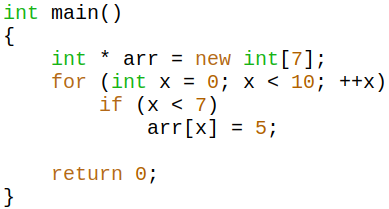
\includegraphics[]{predicates-improvement.png}
    \caption{Цикл с дополнительным условием внутри: C++}
    \label{fig:predicates-improvement-cpp}
\end{figure}

\begin{figure}
    \inputTikZ{predicates-improvement}
    \caption{Цикл с дополнительным условием внутри: SSA форма}
    \label{fig:predicates-improvement-ssa}
\end{figure}

В цикле, представленном на
рисунке~\ref{fig:predicates-improvement-cpp} значение переменной $x$,
использующейся как индекс при записи в массив, дополнительно
ограничено числом $7$. Таким образом, значение счётчика цикла
находится в диапазоне $[0, 9]$, однако значение индекса не превышает
$7$. Программа в SSA форме представлена на
рисунке~\ref{fig:predicates-improvement-ssa}.

Проблема подхода~\cite{li2010practical} состоит в правиле,
определяющем, какие предикаты должны учитываться при вычислении use
range переменной $v$ в инструкции $P$. Во-первых, условный переход,
использующий предикат, должен доминировать инструкцию $P$, то есть все
пути из входа в функцию в $P$ должны проходить через
предикат. Во-вторых, $P$ должна быть достижима только из одного
потомка условного перехода. Однако, как нетрудно видеть из
рисунка~\ref{fig:predicates-improvement-ssa}, в данном случае
инструкция записи в массив достижима из обоих потомков условного
перехода. Это приводит к тому, что условие $x < 7$ не применяется для
вычисления use range $x$ в месте записи в массив, из-за чего
анализатор выдаёт несуществующую ошибку.

Описанная проблема может быть решена модификацией второго правила,
определяющего, должен ли учитываться предикат при вычислении use
range. Модифицированное правило ослабляет требование, что инструкция
$P$ должна быть достижима только из одного потомка условного перехода,
использующего предикат. Ослабленное требование заключается в том, что
должен быть ровно один потомок $S$ условного перехода $C$, такой что
$P$ достижима из $C$, игнорируя все рёбра из $C$, кроме
$C \rightarrow S$. В таком случае условие, соответствующее переходу в
$S$, считается выполненым.

Покажем, что предложенная модификация сохраняет
корректность. Рассмотрим произвольный путь в инструкцию $P$. По
первому правилу $P$ доминируется $C$, а значит, путь обязан пройти
через $C$. Рассмотрим последнее ребро на этом пути, исходящее из
$C$. Пусть это ребро $C \rightarrow T$. Если $T = S$, значит, условие,
соответствующее переходу в $S$, выполнено, что и требовалось
доказать. Если же $T \neq S$, то путь в $P$ проходит по другому ребру
из $C$, а значит, предположение о том, что ребро $C \rightarrow T$
является последним на пути, неверно.

При использовании модифицированного правила предикат $x < 7$ будет
учтён в месте записи в массив, т. к. из вершины $x_1 = x + 1$ нет
пути, не проходящего по ребру, соответствующему условию $x < 7$. Таким
образом, предложенная модификация позволяет избавиться от ложного
срабатывания в приведённом примере, при этом сохраняя общую
корректность анализа.

\FloatBarrier

\section{Межпроцедурный анализ}

Одним из главных недостатков подхода~\cite{li2010practical} является
отсутствие межпроцедурного анализа. Каждая функция анализируется
независимо, информация о возможных значениях аргументов
игнорируется. На практике программы обычно состоят из большого числа
маленьких функций, и анализа одной изолированной функции недостаточно,
чтобы точно определить, всегда ли обращение к массиву корректно.

В данной работе анализ был расширен до межпроцедурного. Для этого
функции анализируются в порядке топологической сортировки: от
вызывающей к вызываемой. Если в графе вызовов есть цикл, то
топологическая сортировка неопределена, в таком случае цикл
разрывается в случайных местах. При вызове функции в глобальный
контекст программы записываются диапазоны значений (use ranges)
аргументов, передаваемых в функцию. Рассматриваются целочисленные
аргументы, а также указатели, для которых запоминается размер буфера
(массива). При повторном вызове функции диапазоны аргументов
объединяются с уже сохранёнными.  Таким образом, при анализе функции
для её аргументов известны диапазоны возможных значений. Если функция
ни разу не вызывалась, то анализатор считает, что её аргументы могут
принимать любые значения.

\FloatBarrier

\chapterconclusion

В главе 2 представлены результаты исследования алгоритма,
описанного в статье~\cite{li2010practical}. В ходе исследования были
выявлены различные недостатки алгоритма, которым было уделено внимание
в данной работе. Показаны примеры кода, когда алгоритм работает
некорректно, предложены модификации исходного алгоритма, направленные
на устранение выявленных проблем. Доказана корректность предложенных
модификаций.

%-*-coding: utf-8-*-
\chapter{Практическая реализация и результаты}

\section{Реализация}

Предложенный подход был реализован на языке C++.  Как и в
статье~\cite{li2010practical}, было принято решение анализировать не
исходный код на C/C++, а промежуточное представление
LLVM~\cite{lattner2004llvm}. У такого подхода есть несколько весомых
преимуществ~\cite{merz2012llbmc}. Во-первых, LLVM-IR состоит из более
простых языковых конструкций, нежели C или тем более C++, что упрощает
анализ и позволяет охватить большее число возможностей языка с
меньшими усилиями. Во-вторых, код LLVM-IR представляет из себя
результат работы компилятора и является очень близким к тому, что
будет реально выполняться. Это позволяет найти ошибки, появившиеся в
результате трансформаций, выполняемых компилятором. Также
инфраструктура LLVM содержит огромное число встроенных оптимизаций,
средств для анализа и т. п., что можно использовать при
реализации. Ещё одним преимуществом анализа LLVM-IR является то, что
за счёт этого автоматически поддерживается любой язык, для которого
есть компилятор в LLVM-IR, не только C и C++ (являющиеся примерами
таких языков). Также стоит отметить, что программа в LLVM-IR всегда
представлена в SSA форме, на которой базируется описанный ранее
алгоритм. Альтернативное решение состоит в построении SSA формы для
исходной программы на C/C++ и её анализе, однако было показано, что
анализ LLVM-IR имеет существенные преимущества. Язык C++ был выбран
для реализации анализатора преимущественно по двум
причинам. Во-первых, библиотека LLVM написана на C++ и может быть
использована напрямую. Для большого числа популярных языков написаны
интерфейсы вызова сторонних функций библиотеки LLVM, однако они могут
быть неполными или устаревшими. Во-вторых, за счёт использования C++
проще достичь высокой производительности.

Изначально подход из статьи~\cite{li2010practical} был реализован в
полном соответствии с описанием. После этого было проведено
исследование работы алгоритма на различных тестовых примерах, найдены
недостатки и разработаны способы их устранения, описанные в предыдущей
главе.

\subsection{LLVM}

В LLVM каждое значение ($llvm::Value$) идентифицируется обычным
указателем ($llvm::Value *$), поэтому диапазоны переменных
ассоциируются с указателями на значения. Для идентификации инструкций
в рамках use range используются указатели на базовые блоки
($llvm::BasicBlock$), поскольку use range переменной одинаков во всех
инструкциях из одного базового блока. Для выявления инструкций,
выделяющих блоки памяти, использовалась функция $isAllocationFn$ из
LLVM. Размер массива вычисляется как число байт, выделяемых такой
функций, поделённое на размер типа данных в массиве. Информация о
размере типа в байтах также предоставляется LLVM. В качестве
инструкций, обращающихся к памяти, рассматриваются $store$ и
$load$. Анализатор начинает вычисление диапазонов, только встретив
одну из этих инструкций, то есть анализ выполняется «по требованию».

Также LLVM предоставляет полезные функции и классы для расчёта use
range. Для проверки того, что инструкция доминируется предикатным
узлом, необходимой для уточнения use range, используется
$llvm::DominatorTree$, с помощью которого можно проверять предикат
доминируемости. Другая функциональность, необходимая для уточнения
диапазона значений, заключается в проверке достижимости одного
базового блока из другого. В общем случае такая проверка невозможна,
однако в LLVM есть функция $llvm::isPotentiallyReachable$, которая
возвращает $false$, если базовый блок точно недостижим, и $true$ в
противном случае. Как было показано в предыдущей главе, простая
проверка достижимости не является достаточно точной и может приводить
к неправильным результатам. При более точном подходе необходимо
игнорировать рёбра из $C$, кроме ребра $C \rightarrow S$. Поэтому
использовалась модифицированная версия функции, игнорирующая такие
рёбра.

При обнаружении ошибки о ней необходимо сообщить пользователю в
понятном формате. Для этого нужно сопоставлять инструкции из
промежуточного представления LLVM выражениям в исходном коде на
высокоуровневом языке. Эта проблема решается за счёт использования
отладочной информации, генерируемой компилятором при использовании
специального флага. В LLVM такая информация представлена классом
$DebugLoc$. Если программа скомпилирована с отладочной информацией, то
по инструкции LLVM можно получить её $DebugLoc$ и сообщить
пользователю, где в исходном коде находится ошибка.

\subsection{Gated Single Assignment}

Одной из наиболее важных деталей алгоритма является использование
Gated Single Assignment формы
(GSA)~\cite{ottenstein1990program}. Отличие этой формы от SSA
заключается в том, что аргументы $\phi$-инструкций также содержат
условия, которые гарантировано выполняются, если данное значение
возвращается $\phi$-инструкцией. Это позволяет существенно повысить
точность анализа, отбрасывая невозможные значения переменных.

В реализации анализатора использовался алгоритм для конвертации SSA
формы в GSA, описанный в статье~\cite{tu1995efficient}. Данный
алгоритм является одним из наиболее простых в реализации. Он не
требует, чтобы исходная программа была в SSA, однако существенно
упрощается, если это выполнено. В основе алгоритма лежит понятие
«выражение пути» (path expression), которое является регулярным
выражением над алфавитом, состоящем из рёбер в графе потока
управления. Пути, приходящие в $\phi$-инструкцию, представляются
выражениями пути. В конце работы алгоритма выражения пути превращаются
в предикаты GSA-формы. Несмотря на свою простоту, алгоритм также
является более эффективным по сравнению со своими аналогами. В
результате работы алгоритма для каждого операнда каждой
$\phi$-инструкции известен определённый набор условий, который должны
выполняться, чтобы данное значение было результатом
$\phi$-инструкции. После этого вычисленные условия применяются для
уточнения диапазонов значений $\phi$-инструкций в месте их определения.

\subsection{Символьные вычисления}

TODO

\subsection{Обработка больших программ}

Одной из главных проблем при обработке больших программ, состоящих из
большого числа файлов и сложного механизма сборки, является
необходимость скомпилировать программу в LLVM-IR. Для решения проблемы
используется утилита whole-program-llvm~\cite{wllvm}, написанная на
языке Python, которая используется также в проекте
KLEE~\cite{cadar2008klee}. Утилита подменяет компилятор (gcc или
clang) обёртками, которые помимо компиляции кода также сохраняют
дополнительную служебную информацию о расположении кода в генерируемых
файлах. При линковке объектных файлов служебная информация
объединяется. Таким образом, получающийся в результате сборки
исполняемый файл (или библиотека) содержит всю необходимую информацию
для восстановления биткода. На последнем шаге из файла извлекается
биткод, соответствующий всей программе целиком. При этом сохраняется
отладочная информация, если она была сгенерирована компилятором. В
дальнейшем биткод полностью передаётся анализатору. Поскольку утилита
является простой обёрткой над компилятором, её очень легко
использовать с различными системами сборки, такими как
GNU~Make~\cite{gnumake}. Достаточно лишь верно указать используемый
компилятор.

\section{Экспериментальные результаты}

TODO

\section{Сравнение}

Также было проведено сравнение анализатора с другими доступными
анализаторами C/C++ кода. Использовались следующие анализаторы: Clang
Analyzer, CppCheck, PVS-Studio, Splint, а также реализация
анализатора, описанного в статье~\cite{li2010practical}, и реализация
предложенного подхода. Для сравнения использовался набор синтетических
тестов, представленных в листинге~\ref{lst:comparison}.

\begin{table}[!h]
\caption{Результаты сравнения анализаторов}\label{tab:comparison}
\centering
% \begin{tabu}{|*{18}{X[c]|}}\hline
%   --                 & TP  & FP & FN \\\hline
%   Clang Analyzer     & 0   & 0  & 0  \\\hline
%   CppCheck           & 3   & 0  & 9  \\\hline
%   PVS-Studio         & 4   & 0  & 8  \\\hline
%   Splint             & 9   & 3  & 3  \\\hline
%   Li et at.          & 12  & 8  & 0  \\\hline
%   Предложенный метод & 12  & 0  & 0  \\\hline
% \end{tabu}
  \begin{tabular}{|*{18}{c|}}\hline
  --                 & TP  & FP & FN \\\hline
  Clang Analyzer     & 0   & 0  & 0  \\\hline
  CppCheck           & 3   & 0  & 9  \\\hline
  PVS-Studio         & 4   & 0  & 8  \\\hline
  Splint             & 9   & 3  & 3  \\\hline
  Li et at.          & 12  & 8  & 0  \\\hline
  Предложенный метод & 12  & 0  & 0  \\\hline
  \end{tabular}
\end{table}

В таблице~\ref{tab:comparison} представлены результаты сравнения.

\chapterconclusion

В данной главе была вкратце описана реализация предложенного
подхода. Приведены экспериментальные результаты запуска анализатора на
крупных проектах. Показано, что анализатор способен находить в них
ошибки, работая за приемлимое время. Также было проведено сравнение с
доступными статическими анализаторами C/C++ кода на наборе тестов,
представленных в листинге~\ref{lst:comparison}. Продемонстрировано
превосходство над представленными анализаторами на данном наборе
тестов.


%% Макрос для заключения. Совместим со старым стилевиком.
\startconclusionpage

%-*-coding: utf-8-*-

Как было показано в данной работе, задача поиска выходов за пределы
динамического массива в C/C++ является крайне актуальной и
представляет практический интерес. Были рассмотрены различные подходы
к решению данной задачи, выделены основные характеристики различных
подходов. За основу был взят подход, описанный в
статье~\cite{li2010practical}.

В ходе работы было проведено детальное исследование
подхода~\cite{li2010practical}, выявлены и продемонстрированы
различные недостатки. Были предложены способы устранения выявленных
недостатков, показана корректность этих способов.

Алгоритм был реализован на языке C++. В результате экспериментов было
показано, что анализатор способен находить ошибки в крупных проектах и
работает за разумное время. Несмотря на наличие ложных срабатываний,
такой анализатор является полезным инструментом разработчика, особенно
операционных систем и сетевых программ. Также было проведено сравнение
с доступными анализаторами. Показано, что реализованный подход
работает лучше промышленных анализаторов, а также лучше базового
подхода, предложенного в \cite{li2010practical}.

Разработанное средство статического анализа было внедрено в проекте
«IoT Devices», реализуемом ООО~«Интеллектуальные системы».

\FloatBarrier


%% Обратите внимание на heading. Без него тоже работает, но название будет другим.
\printmainbibliography

\end{document}
